\documentclass{standalone}
\usepackage{amsmath}
\usepackage{tikz}

\begin{document}
\begin{tikzpicture}
\node (P) at (0,0) {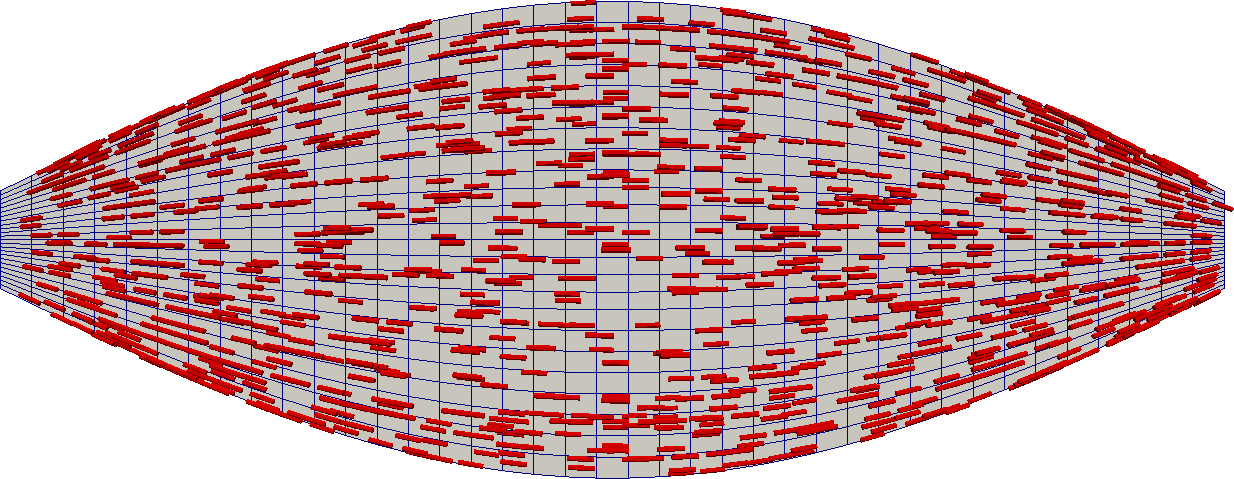
\includegraphics[width=10cm]{./biceps-geometry.png}};
\begin{scope}[scale=0.075]
  \foreach \y in {-5,-2.5,...,5} 
    {
      \draw[->, red, thick] (+67,\y) -- (+75,\y) {};
      \draw[-, black, very thick] (-67,\y) -- (-71,\y-1.5) {};
    }
  \draw[-, black, very thick] (-67.25,-5) -- (-67.25,+5) {};
\end{scope}

\begin{scope}[xshift=-160]
  \node[rotate=90] at (0,0) {$\overline{\boldsymbol{\varphi}} \left( t \right)$};
\end{scope}
\begin{scope}[xshift=170]
  \node[rotate=-90] at (0,0) {$\mathbf{\overline{t}\phantom{}^{\textnormal{mech}}} \left( t \right)$};
\end{scope}
\end{tikzpicture}
\end{document}